\documentclass{beamer}

% Theme and color setup
\usetheme{Madrid}
\usecolortheme{seahorse}
\definecolor{myblue}{RGB}{0, 102, 204}
\setbeamercolor{structure}{fg=myblue}
\setbeamercolor{block title}{bg=myblue!50}
\setbeamercolor{block body}{bg=myblue!10}

\setbeamertemplate{theorems}[numbered] % enables numbering

\newtheorem{proposition}{Proposition}
\numberwithin{proposition}{section}

\usepackage[T1]{fontenc}
\usepackage{amsmath}

% \usefonttheme[onlymath]{serif}
\usefonttheme{serif}

\usepackage{subcaption}
\usepackage{tikz}
\usetikzlibrary{decorations.pathreplacing}
\usetikzlibrary{calc}
\usetikzlibrary {bending,positioning}

\usepackage{adjustbox}

\usepackage[backend=bibtex,style=authoryear,citestyle=authoryear-comp,maxnames=1]{biblatex}
% redefine cite macro
\renewbibmacro*{cite}{%
  \printtext[bibhyperref]{%
    [\printnames[last]{labelname}~\printfield{year}]%
  }%
}
\addbibresource{biblio/Noise2Noise.bib}
% \nocite{*}

\graphicspath{{images/}}

% Title and author information
\title[]{Statistical self-supervised methods to solve linear inverse problem and application to PET reconstruction.}
\author{Bouchez-Delotte Sacha}
% \institute{Your Institution}
\date{\today}

\begin{document}

% Title slide
\begin{frame}
    \titlepage
\end{frame}

\begin{frame}{Table of contents}
    \tableofcontents
\end{frame}

\section{Context}

%

\begin{frame}{Doctoral project goals}{Positron Emission Tomography (PET) imaging}
    \begin{columns}
        \begin{column}{0.5\textwidth}
            \begin{itemize}
                \item \textbf{PET} is a medical imaging technique that detects pairs of gamma rays emitted by a tracer.
                \item The patient is injected with a radioactive tracer that emits positrons.
                \item When a positron meets an electron, they annihilate, producing two gamma photons detected by a ring of detectors.
                \item The data collected is used to reconstruct images of tracer concentration in the body.
            \end{itemize}
        \end{column}
        \begin{column}{0.5\textwidth}
            \centering
            % PET principle illustration (already present)
             \begin{figure}
                    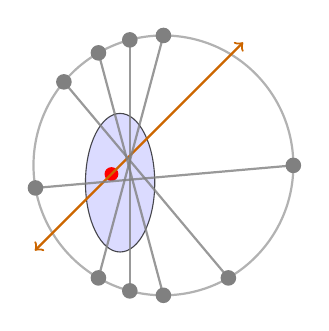
\begin{tikzpicture}[scale=1.1]
                        % PET scanner ring
                        \draw[thick, gray!60] (0,0) circle (1.5);
                        % Patient ellipse
                        \draw[fill=blue!20, opacity=0.7] (-0.5,-0.2) ellipse (0.4 and 0.8);
                        % Emission point
                        \fill[red] (-0.6,-0.1) circle (0.08);
                        % Gamma rays from emission point (aligned, opposite directions)
                        \draw[->, thick, orange!80!black] (-0.6,-0.1) -- ++(45:2.15);
                        \draw[->, thick, orange!80!black] (-0.6,-0.1) -- ++(225:1.25);
                        % Coincident green points at irregular locations
                        \foreach \i/\a/\b in {
                              1/0/190,
                              2/90/240,
                              3/105/255,
                              4/120/270,
                              5/140/300
                        } {
                            % Place green points on the ring
                            \fill[black!50] ({1.5*cos(\a)}, {1.5*sin(\a)}) circle (0.09);
                            \fill[black!50] ({1.5*cos(\b)}, {1.5*sin(\b)}) circle (0.09);
                            % Draw coincident line (not perfectly intersecting)
                            \draw[thick, black!50, opacity=0.8] ({1.5*cos(\a)}, {1.5*sin(\a)}) -- ({1.5*cos(\b)}, {1.5*sin(\b)});
                        }
                    \end{tikzpicture}
            \caption{PET : Emission event detected by ring detectors}
            \end{figure}

        \end{column}
    \end{columns}
\end{frame}


\begin{frame}{PET reconstruction as a linear inverse problem}{Context}
    \centering $\vcenter{\hbox{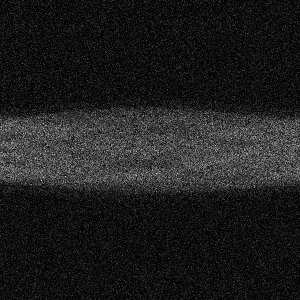
\includegraphics[scale=0.25]{simu_pt.jpg}}}
= \text{Poisson}\left( A \cdot
\vcenter{\hbox{
\includegraphics[scale=0.5, trim = 20 20 20 20, clip]{gt_web_after_scaling.png}}}
\right) $
\vspace{0.5cm}
    \begin{itemize}
        \item The PET reconstruction problem can be formulated as a Poisson linear inverse problem :
        \begin{equation}
            Y | X=x\sim \text{Poisson}(Ax)
        \end{equation}
        \item $A$ is \textbf{known} and is the \textbf{system/projection matrix}.
    \end{itemize}
\end{frame}

\begin{frame}{PET : Some SOTA reconstruction methods}{Context}
    \begin{columns}
        \begin{column}{0.65\textwidth}
            \begin{itemize}
                \item Iterative statistical reconstruction methods
                \begin{itemize}
                    \item Maximum Likelihood-Based (e.g. MLEM, OSEM)
                    \item Penalized Likelihood-Based (e.g. MAPEM)
                \end{itemize}
                \item Analytical reconstruction methods (e.g. FBP)
                \item Machine Learning / Deep Learning methods
                \begin{itemize}
                    \item Post-Reconstruction enhancement (e.g. CNN denoising)
                    \item Direct reconstruction (e.g. end-to-end CNN)
                \end{itemize}
            \end{itemize}
        \end{column}
        \begin{column}{0.35\textwidth}
            \begin{figure}
                \begin{tikzpicture}
                    % put image in node
                    \node (brain) {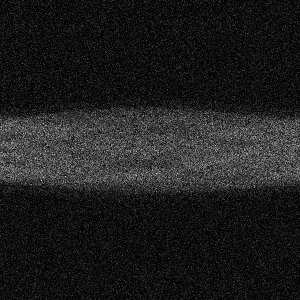
\includegraphics[scale=0.2]{simu_pt.jpg}};

                    \node (sino) [below=of brain] {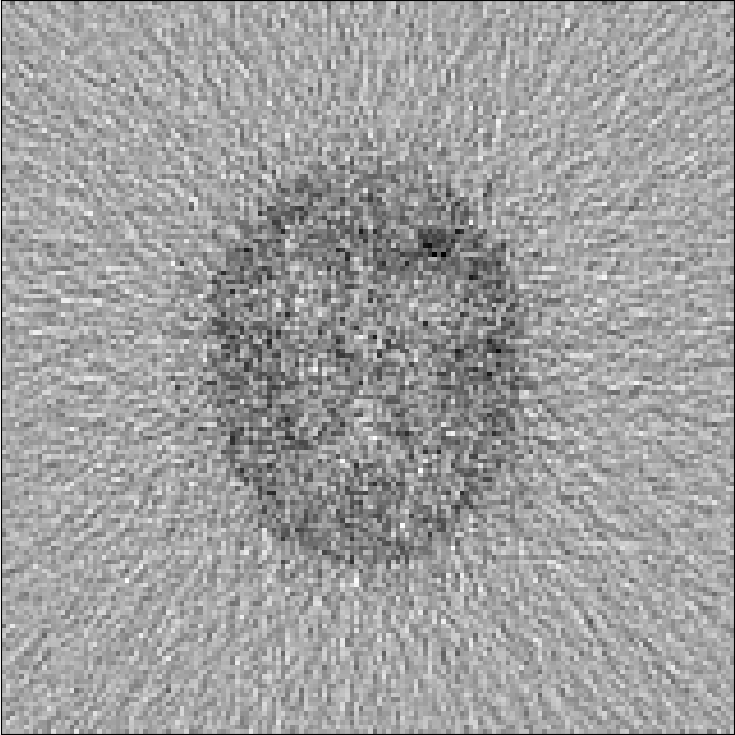
\includegraphics[scale=0.125, trim=100 100 100 100, clip]{image_to_image/brain_0.png}};

                    \draw[->, thick] (brain) -- (sino) node[midway, fill=white] {Reconstruction (FBP)};
                \end{tikzpicture}
            \end{figure}
        \end{column}
    \end{columns}

\end{frame}

\begin{frame}{PET : ground truth unavailability}{Context}

    \begin{figure}
        \begin{columns}
            \begin{column}{0.3\textwidth}
                \centering
                \begin{adjustbox}{max totalsize={\textwidth}{0.8\textheight}}
                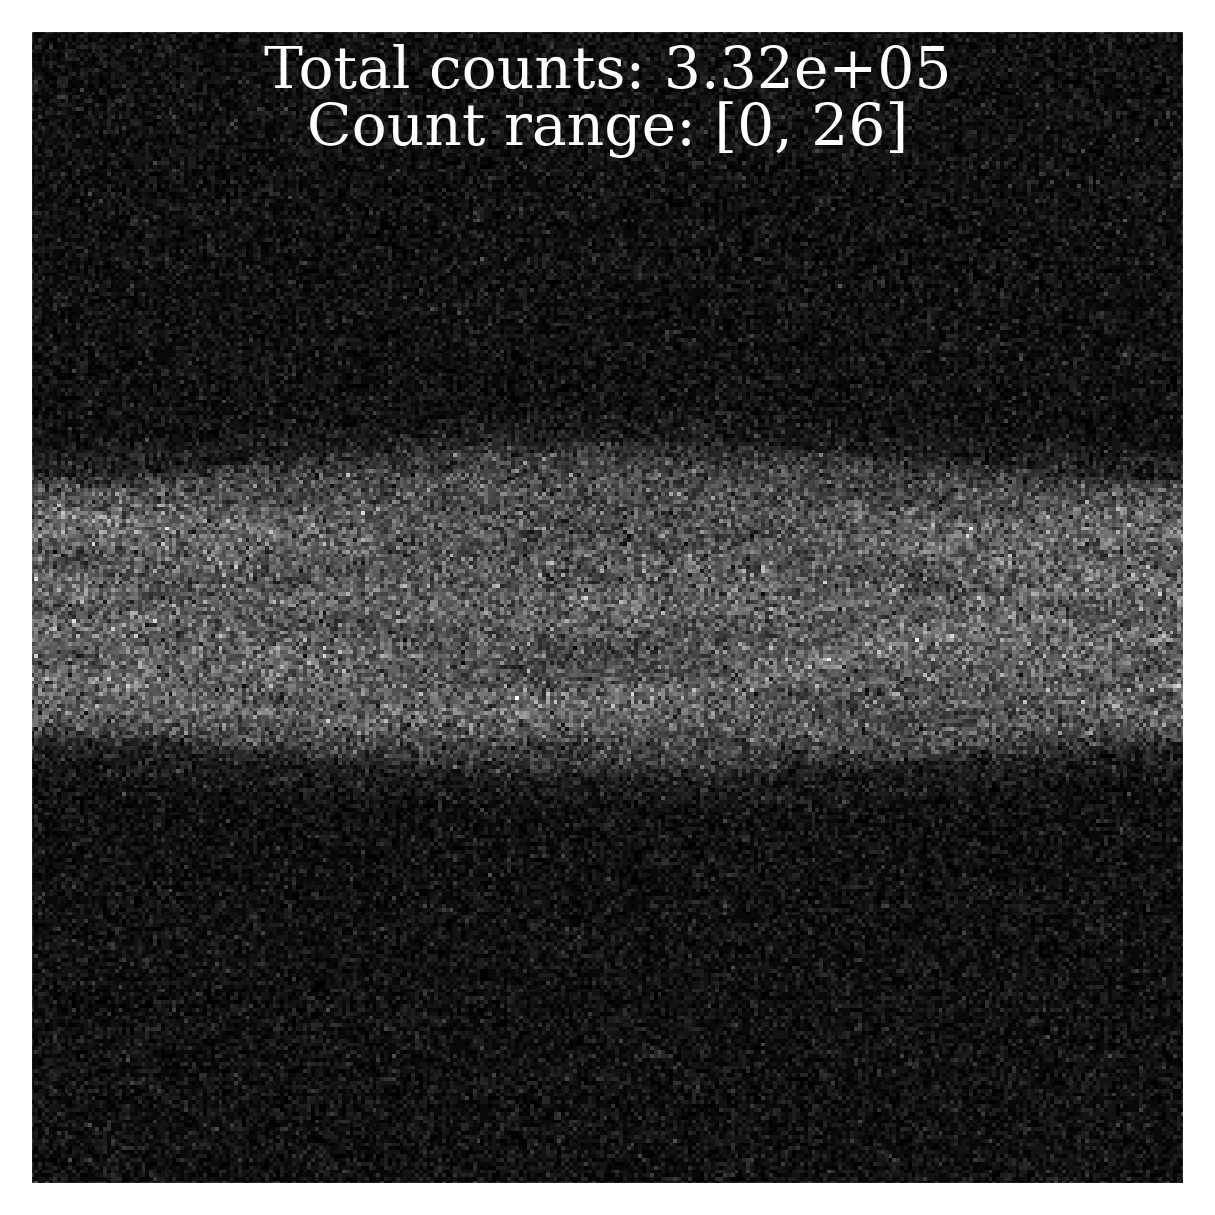
\includegraphics{prompt_03M.png}
                \end{adjustbox}
            \end{column}
            \begin{column}{0.3\textwidth}
                \centering
                \begin{adjustbox}{max totalsize={\textwidth}{0.8\textheight}}
                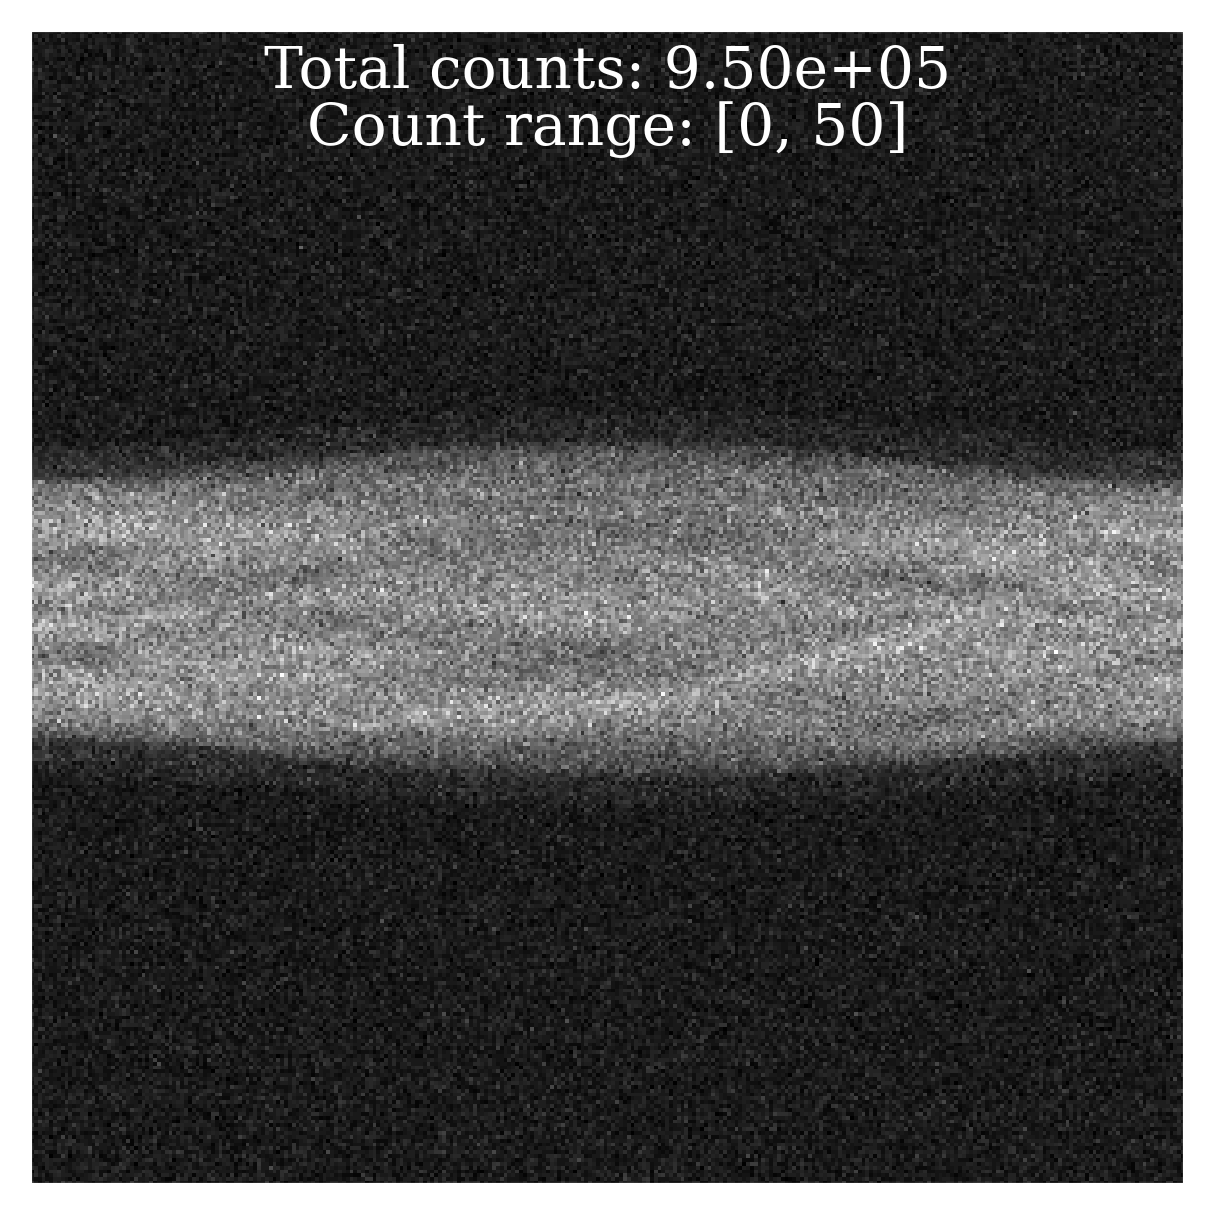
\includegraphics{prompt_1M.png}
                \end{adjustbox}
            \end{column}
            \begin{column}{0.3\textwidth}
                \centering
                \begin{adjustbox}{max totalsize={\textwidth}{0.8\textheight}}
                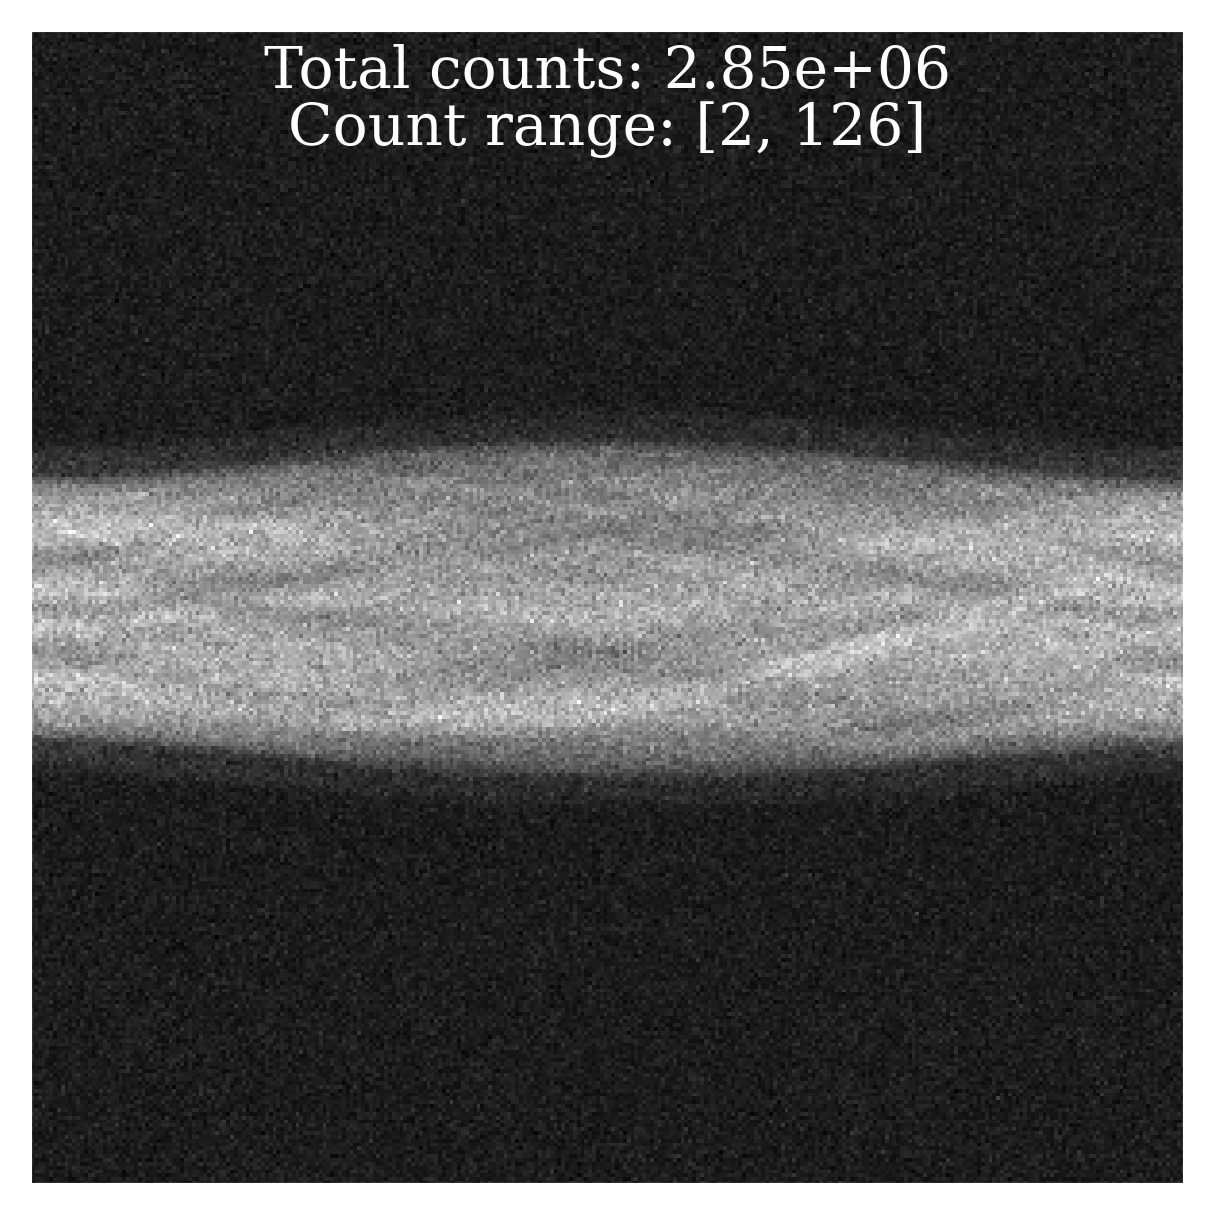
\includegraphics{prompt_3M.png}
                \end{adjustbox}
            \end{column}
        \end{columns}
    \caption{PET : Noisy prompt sinograms with different count levels}
    \end{figure}

    \begin{itemize}
        \item Raw data is noisy and reference high-count sinograms (right) are less available.
        \item Ground truth images are not available at all.
    \end{itemize}
    
\end{frame}




\section{Noise2Noise : restore image without clean data}


\begin{frame}{The classical supervised framework}{Noise2Noise : restore image without clean data}
    
    \begin{itemize}
        \item $x$ is known ; samples are pairs of \textbf{noisy} measurement and \textbf{clean} image $(y, x)$.
        \item We want to learn a mapping $f_\theta(y) \approx x$.
    
    \begin{equation}
        \mathcal{L}(\theta) = \frac{1}{N} \sum_{i=1}^N \rho\left(f_\theta\left(y_i\right) - x_i\right)
        \label{supervised_loss}
    \end{equation}

    \end{itemize}


    \begin{itemize}
        \item Lack of ground truth data, especially in the medical field.
    \end{itemize}

\end{frame}




\begin{frame}{The Noise2Noise insight}{Noise2Noise : restore image without clean data}
    
    \begin{itemize}
        \item Samples are pairs of \textbf{noisy} measurements $(y^{(1)}, y^{(2)})$ of the same \textbf{unknown} underlying image $x$.

        \item We want to learn a mapping $Af_\theta(y^{(1)}) \approx y^{(2)}$ \cite{xia_training_nodate}, hence the following objective function :
    
    \begin{equation}
        \mathcal{L}(\theta) = \frac{1}{N} \sum_{i=1}^N \rho\left(Af_\theta\left(y_i^{(1)}\right) - y_i^{(2)}\right)
        \label{n2n_loss}
    \end{equation}

    \item Note that $A = \text{Id}$ is the original Noise2Noise formulation  \cite{lehtinen_noise2noise_2018} and is pure denoising.

    \end{itemize}

\end{frame}





\begin{frame}{Statistical conditions}{Noise2Noise : restore image without clean data}


    \begin{itemize}
        \item We will consider the following statistical conditions :
        \begin{equation}
            \begin{cases}
                \mathbb{E} \left[Y_i | X=x\right] = Ax & \text{(centered noise)} \\
                Y_1 | X \perp\!\!\!\!\perp Y_2 | X & \text{(independancy)}
            \end{cases}
        \label{statistical-conditions}
        \end{equation}
    \end{itemize}

    \begin{proposition}
        Under the statistical conditions \ref{statistical-conditions}, the optimal solution of the Noise2Noise loss \ref{n2n_loss} is the same as the optimal solution of the supervised loss for some good choice of $\rho$ as $N \to \infty$.
        \label{n2n-prop}
    \end{proposition}
\end{frame}




\begin{frame}{Statistical conditions}{Noise2Noise : restore image without clean data}

    \begin{proposition}
        If $\rho$ is the $L_2$ loss, then proposition \ref{n2n-prop} is satisfied and the optimal solution is the \textbf{mean} of noise realisations.
         \label{n2n-prop-l2}
    \end{proposition}

    \begin{proposition}
        If $\rho$ is the $L_1$ loss, then proposition \ref{n2n-prop} is satisfied and the optimal solution is the \textbf{median} of noise realisations.
         \label{n2n-prop-l1}
    \end{proposition}

    \begin{proposition}
        If noise is poissonian (Y | X=x $\sim \mathcal{P}(x)$) and $\rho$ is the \textbf{Poisson Negative Log-Likelihood} ($\rho(y^{(1)}, y^{(2)}) = \sum_i y_i^{(1)} \log(y_i^{(2)}) - y_i^{(2)}$), then proposition \ref{n2n-prop} is satisfied.
         \label{n2n-prop-kl}
    \end{proposition}
\end{frame}


\begin{frame}{Further intuition}{Noise2Noise : restore image without clean data}
    \centering
    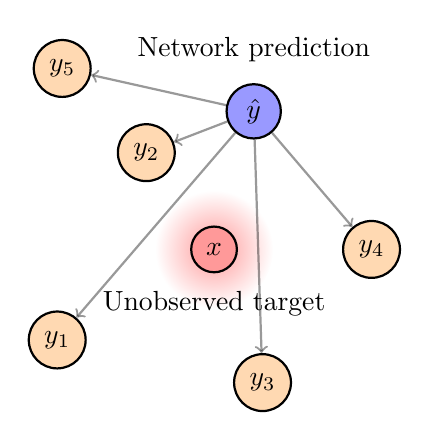
\begin{tikzpicture}
        % Network prediction node
        \node [draw, circle, fill=blue!40, thick] (pred) {\textbf{$\hat{y}$}};
        \node [above=0.15cm] at (pred.north) {Network prediction};

        % Clean target node (not directly used, but for reference)
        \node [shade, inner color=red!40, outer color=white, draw=none] (clean_target_halo) at ([xshift=-0.25cm, yshift=-1.5cm]pred.south west) [circle, minimum size=1.5cm] {};
        \node [draw, circle, fill=red!40, thick] (clean_target) at (clean_target_halo)  {\textbf{$x$}};
        \node [below=0.1cm] at (clean_target.south) {Unobserved target};

        % Multiple noisy targets
        \foreach \i/\angle/\distance in {1/210/2.3, 2/125/1.5, 3/290/1.8, 4/0/2, 5/130/3} {
            \node[draw, circle, fill=orange!30, thick] (noisy\i) at ($(clean_target) + (\angle:\distance)$) {\textbf{$y_{{\i}}$}};
            \draw[->, thick, opacity=0.4] (pred) -- (noisy\i);
        }
    \end{tikzpicture}
    % \small
    % \textbf{Noise2Noise:} The network learns from multiple noisy targets, each providing a different noisy realization, and the average prediction converges to the clean signal if noise is zero-mean and independent.
\end{frame}

\begin{frame}{Binomial sampling}{Noise2Noise : restore image without clean data}

    \begin{proposition}
        $Y|X$ is $2$-divisible.

        For instance, $Y_i | X=x \sim \text{Binomial}(Ax, \frac{1}{2})$ works and :
        \begin{equation}
            \begin{cases}
                Y_i | X \sim \text{Poisson}(\frac{1}{2}Ax) \\
                Y_1 | X \perp\!\!\!\!\perp Y_2 | X.
            \end{cases}  
        \end{equation}

        Hence, statistical conditions \ref{statistical-conditions} are satisfied and Noise2Noise can be applied.
         \label{n2n-prop-divisible}
    \end{proposition}

    In the Noise2Noise world, this is called "Recorrupted2Recorrupted" \cite{pang_recorrupted--recorrupted_2021}.
\end{frame}

\section{Applications}

\begin{frame}{Denoising in count domain}{Applications}
    \centering
    \begin{tikzpicture}
        \tiny
        \node (full_sino) {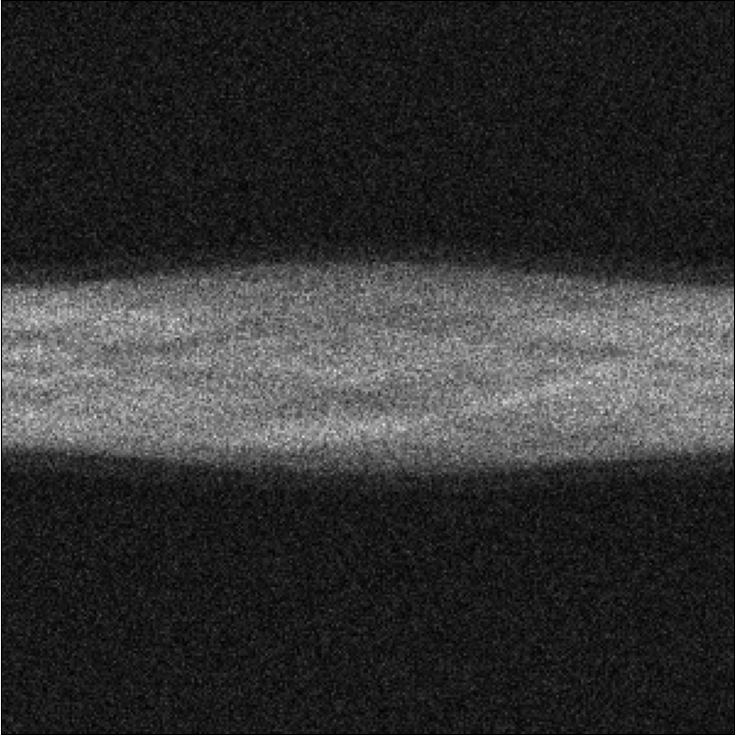
\includegraphics[scale=0.07]{photon_to_photon/sino_bin_0+1.png}};
        \node [right=0.1cm of full_sino] {Sampling};
        \node (bin0) [right=0.45cm of full_sino, yshift=-1.5cm] {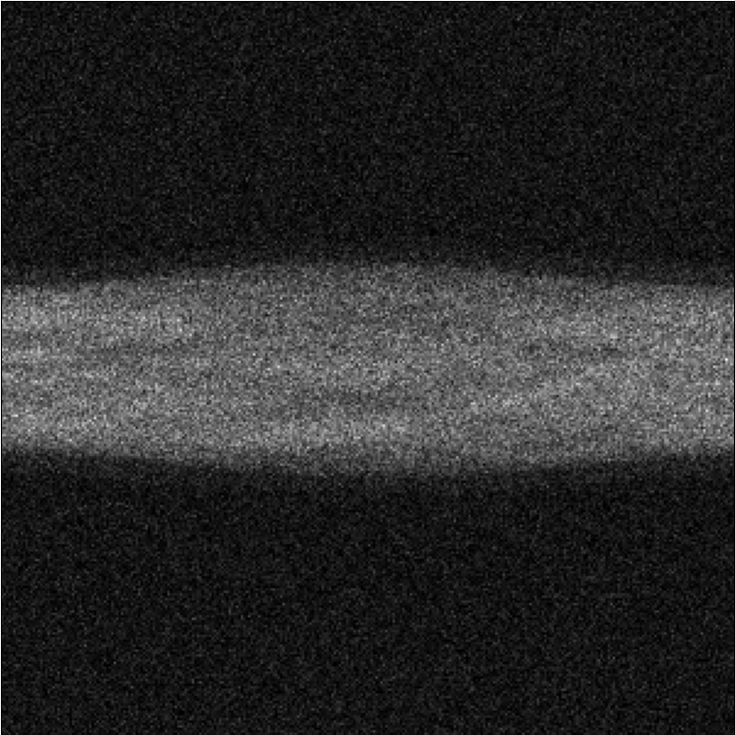
\includegraphics[scale=0.07]{photon_to_photon/sino_bin_0.png}};
        \node (bin1) [right=0.45cm of full_sino, yshift=1.5cm] {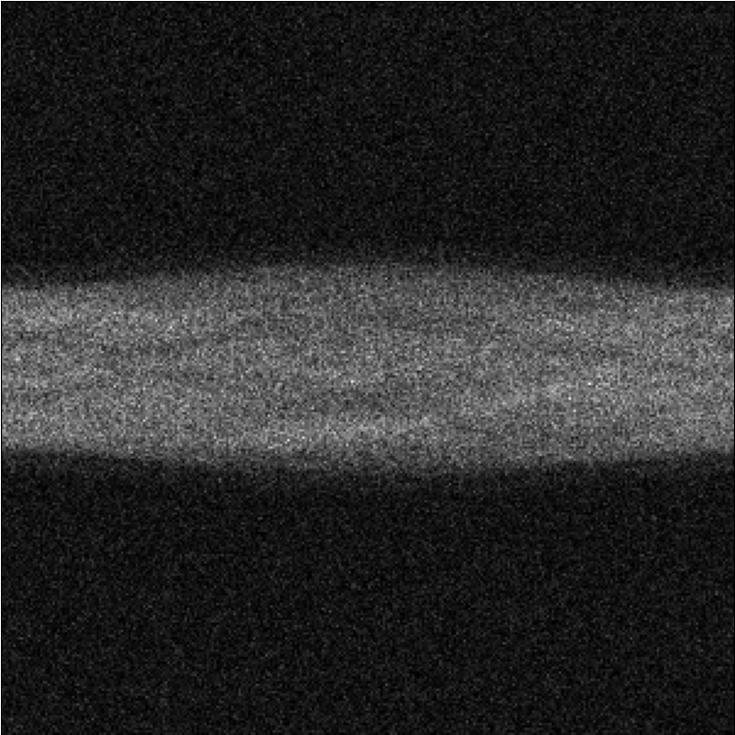
\includegraphics[scale=0.07]{photon_to_photon/sino_bin_1.png}};

        \node (denoised_bin_0) [right=0.45cm of bin0] {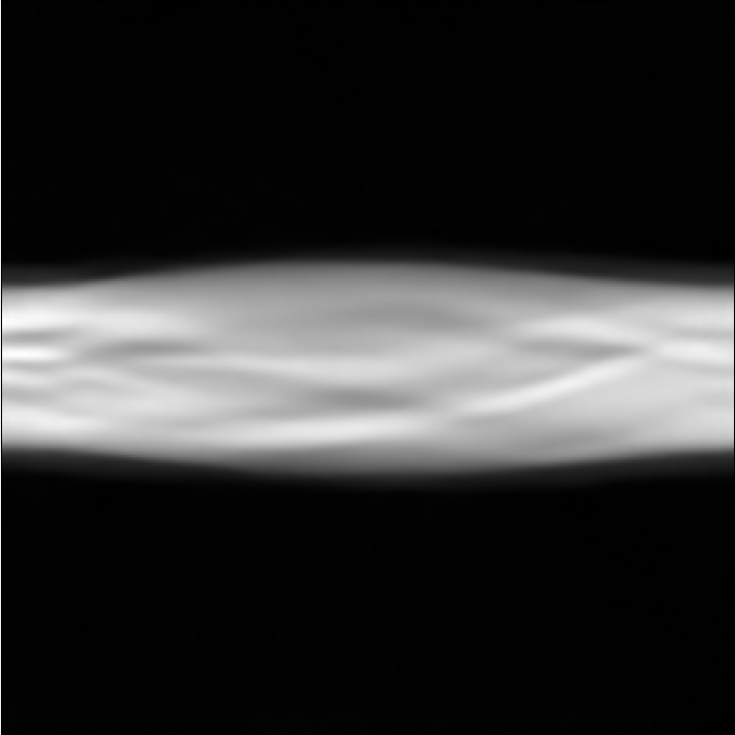
\includegraphics[scale=0.07]{photon_to_photon/sino_bin_0_denoised.png}};
        \node (denoised_bin_1) [right=0.45cm of bin1] {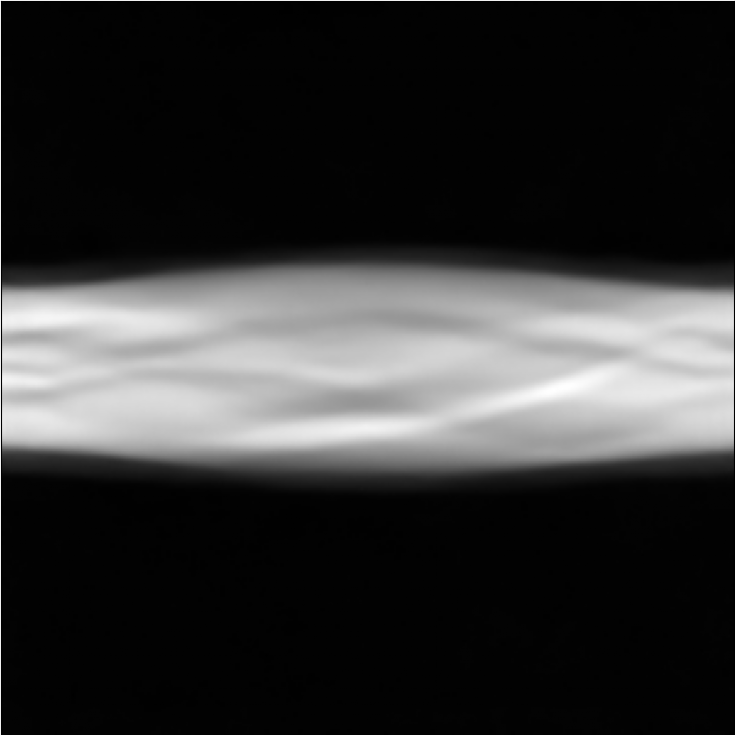
\includegraphics[scale=0.07]{photon_to_photon/sino_bin_1_denoised.png}};

        \node (recon_bin_0) [right=0.45cm of denoised_bin_0] {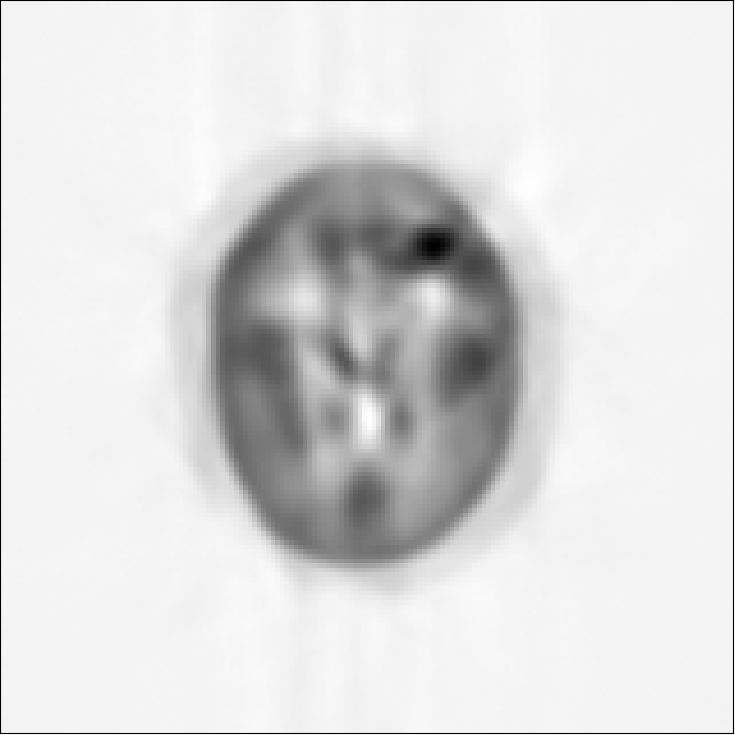
\includegraphics[scale=0.07]{photon_to_photon/brain_bin_0.png}};
        \node (recon_bin_1) [right=0.45cm of denoised_bin_1] {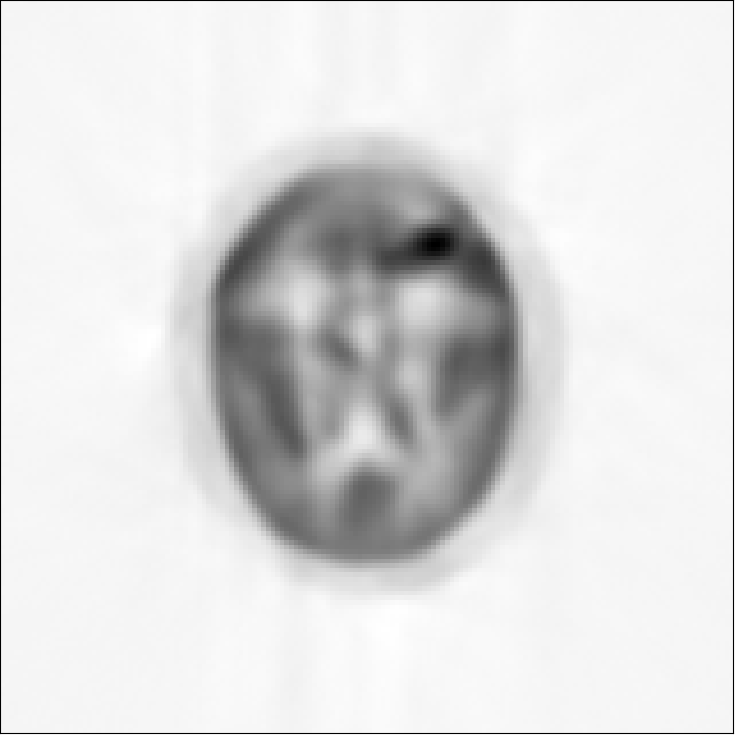
\includegraphics[scale=0.07]{photon_to_photon/brain_bin_1.png}};

        \node (recon_full) [right=0.45cm of recon_bin_1, yshift=-1.5cm] {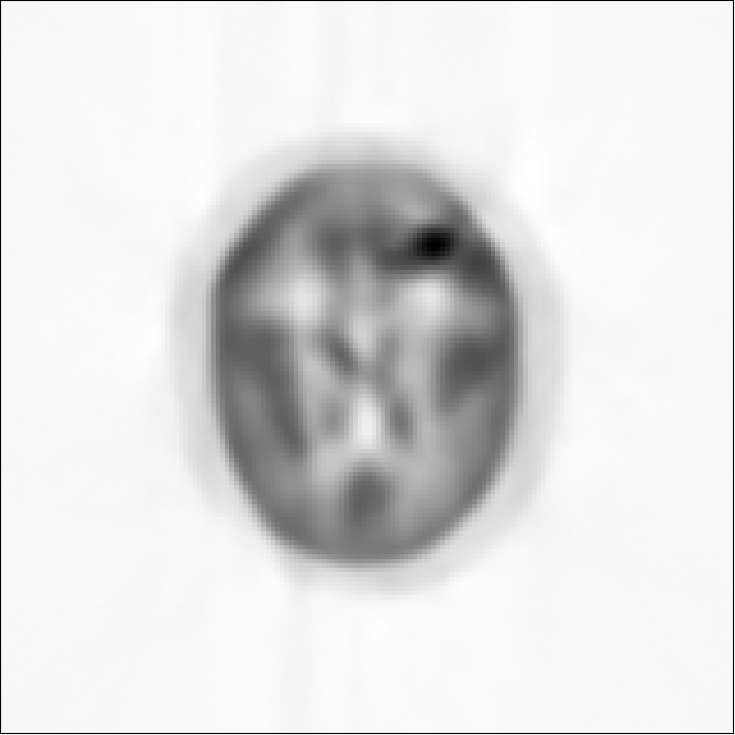
\includegraphics[scale=0.07]{photon_to_photon/brain_bin_0+1.png}};

        \draw[->, thick] (full_sino) -- (bin0);
        \draw[->, thick] (full_sino) -- (bin1);
        \draw[->, thick] (bin0) -- (denoised_bin_0) node[midway, below] {CNN};
        \draw[->, thick] (bin1) -- (denoised_bin_1) node[midway, above] {CNN};
        \draw[->, thick] (denoised_bin_0) -- (recon_bin_0) node[midway, below] {FBP};
        \draw[->, thick] (denoised_bin_1) -- (recon_bin_1) node[midway, above] {FBP};
        \draw[->, thick] (recon_bin_0) -- (recon_full);
        \draw[->, thick] (recon_bin_1) -- (recon_full);

        \draw[<->, thick, orange] (denoised_bin_0.north) -- (bin1.south) node[midway, above, fill=white, inner sep=1pt, yshift=0.15cm] {$\mathcal{L}_{\text{n2n}}$};
        \draw[<->, thick, orange] (denoised_bin_1.south) -- (bin0.north);

    \end{tikzpicture}
\end{frame}


\begin{frame}{Denoising in count domain}{Applications}
    \centering
    \begin{figure}
        
\includegraphics[scale=0.473]{photon_to_photon/results.png}
        \caption{Photon domain training results}
    \end{figure}
\end{frame}

\begin{frame}{Denoising in image domain}{Applications}
    \centering
    \begin{tikzpicture}
        \tiny
        \node (full_sino) {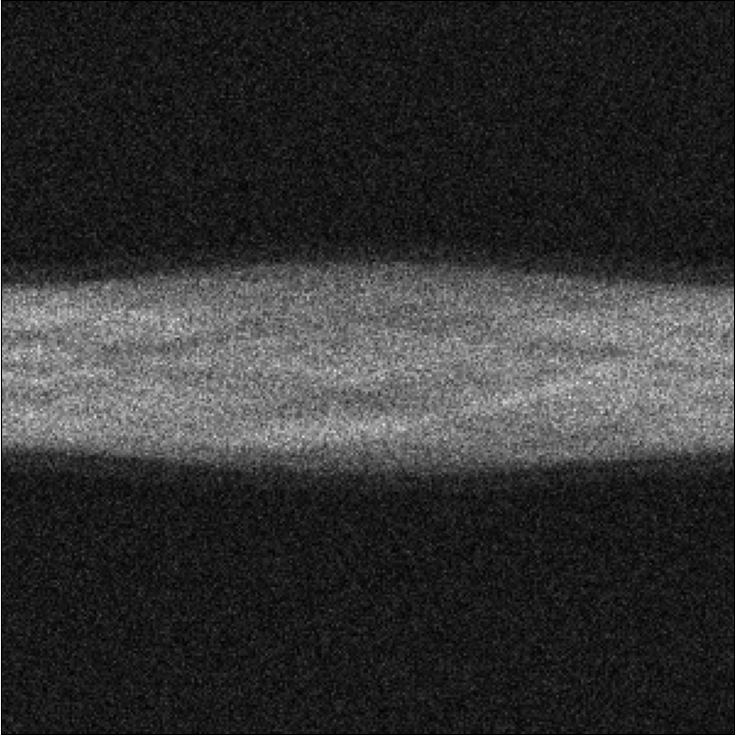
\includegraphics[scale=0.07]{photon_to_photon/sino_bin_0+1.png}};
        \node [right=0.1cm of full_sino] {Sampling};
        \node (bin0) [right=0.45cm of full_sino, yshift=-1.5cm] {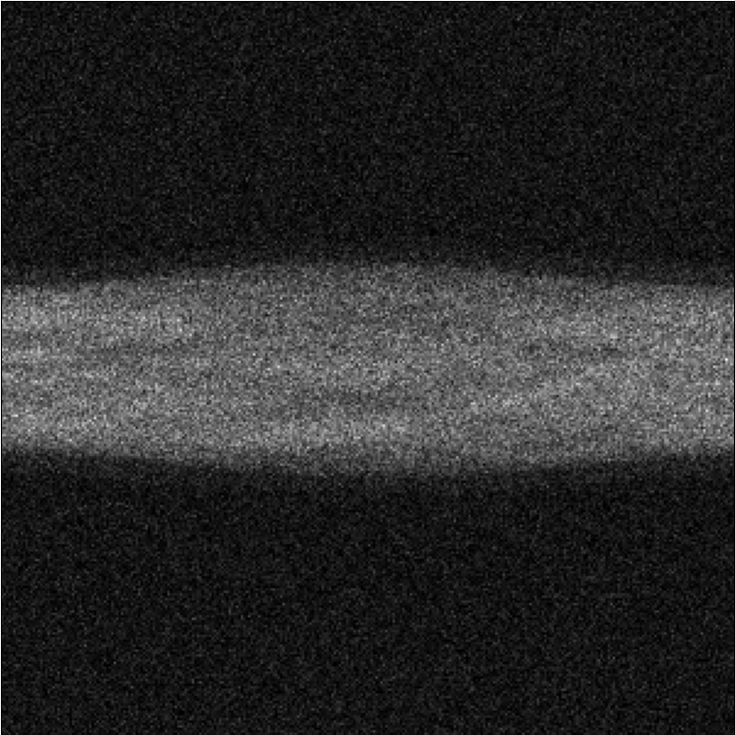
\includegraphics[scale=0.07]{photon_to_photon/sino_bin_0.png}};
        \node (bin1) [right=0.45cm of full_sino, yshift=1.5cm] {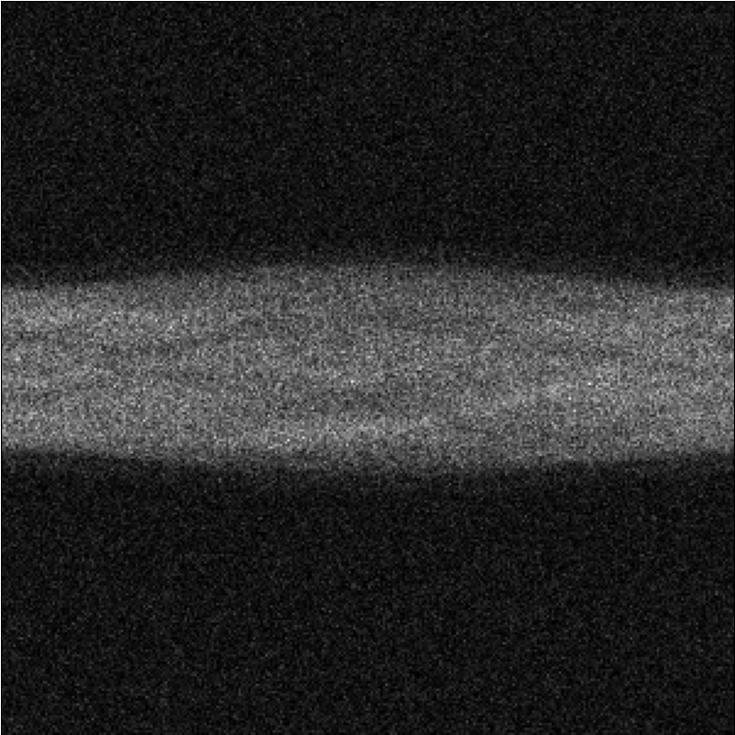
\includegraphics[scale=0.07]{photon_to_photon/sino_bin_1.png}};

        \node (brain_0) [right=0.45cm of bin0] {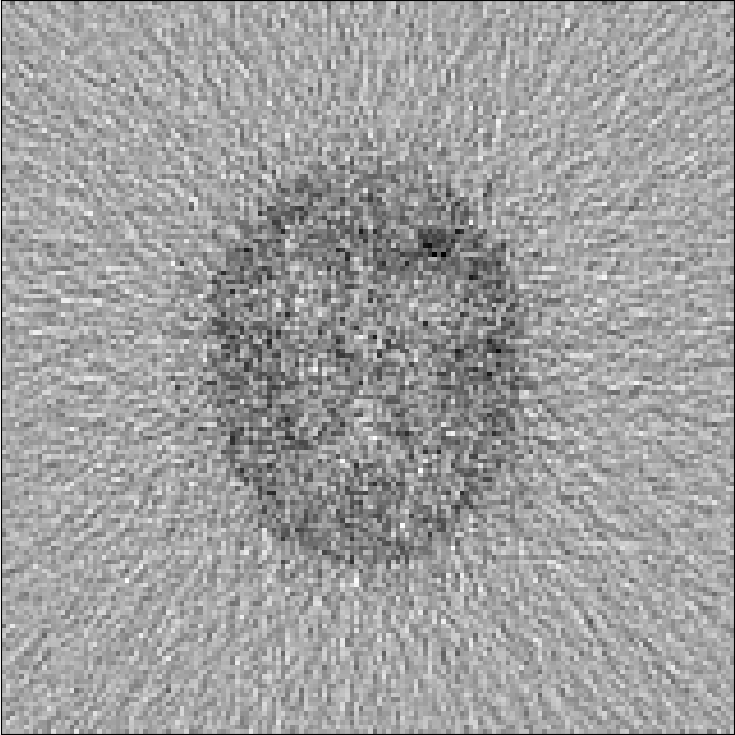
\includegraphics[scale=0.07]{image_to_image/brain_0.png}};
        \node (brain_1) [right=0.45cm of bin1] {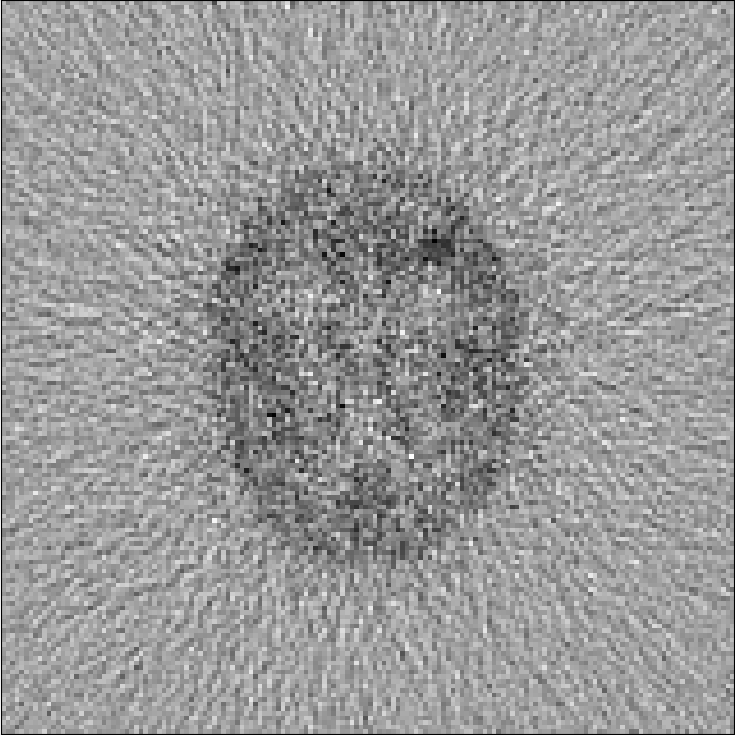
\includegraphics[scale=0.07]{image_to_image/brain_1.png}};

        \node (recon_bin_0) [right=0.45cm of brain_0] {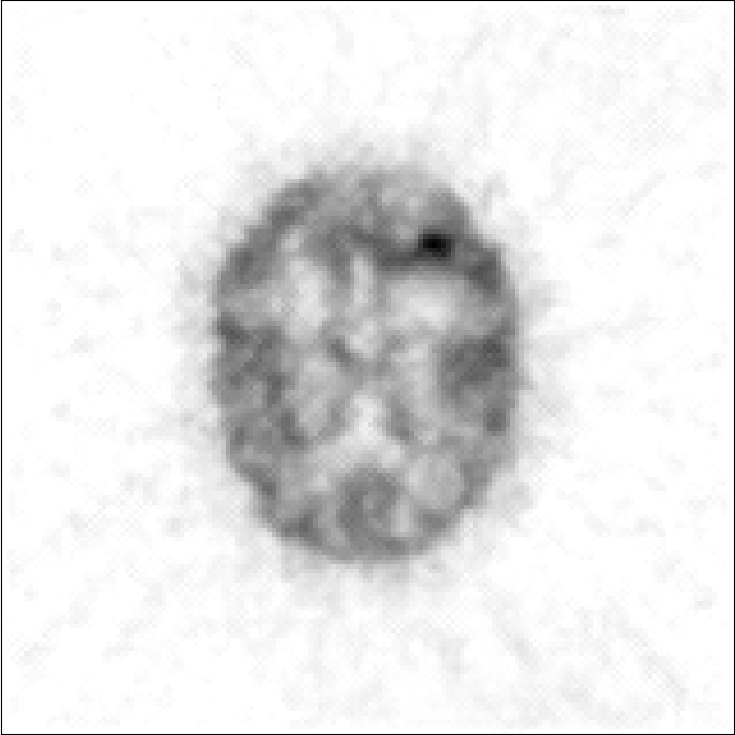
\includegraphics[scale=0.07]{image_to_image/brain_0_denoised.png}};
        \node (recon_bin_1) [right=0.45cm of brain_1] {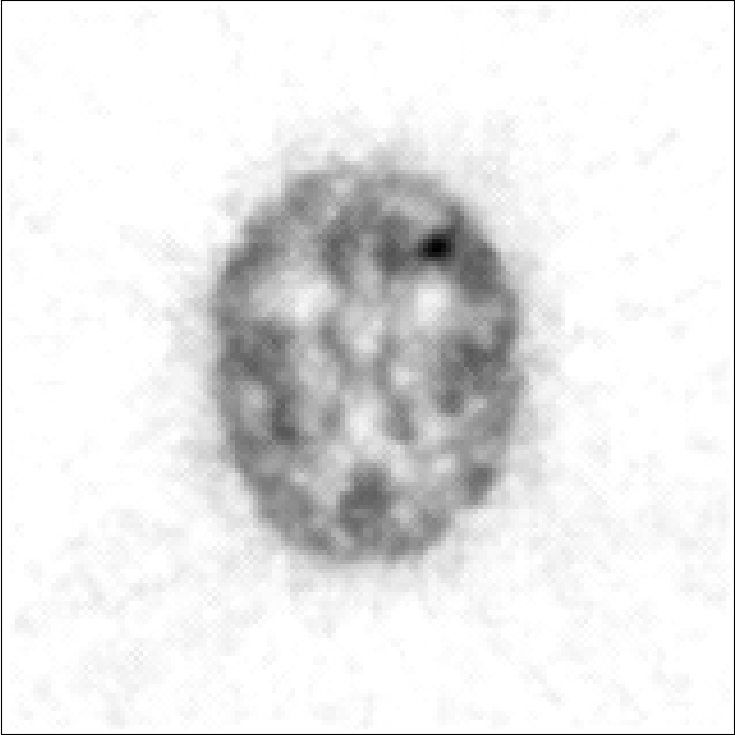
\includegraphics[scale=0.07]{image_to_image/brain_1_denoised.png}};

        \node (recon_full) [right=0.45cm of recon_bin_1, yshift=-1.5cm] {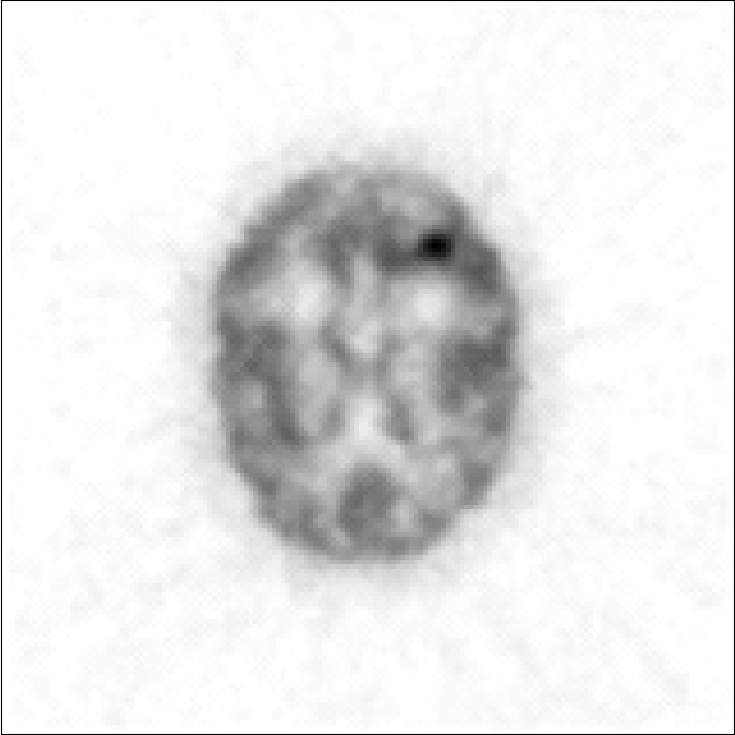
\includegraphics[scale=0.07]{image_to_image/brain_0+1_denoised.png}};

        \draw[->, thick] (full_sino) -- (bin0);
        \draw[->, thick] (full_sino) -- (bin1);
        \draw[->, thick] (bin0) -- (brain_0) node[midway, below] {FBP};
        \draw[->, thick] (bin1) -- (brain_1) node[midway, above] {FBP};
        \draw[->, thick] (brain_0) -- (recon_bin_0) node[midway, below] {CNN};
        \draw[->, thick] (brain_1) -- (recon_bin_1) node[midway, above] {CNN};
        \draw[->, thick] (recon_bin_0) -- (recon_full);
        \draw[->, thick] (recon_bin_1) -- (recon_full);

        \draw[<->, thick, orange] (recon_bin_0.north) -- (brain_1.south) node[midway, above, fill=white, inner sep=1pt, yshift=0.15cm] {$\mathcal{L}_{\text{n2n}}$};
        \draw[<->, thick, orange] (recon_bin_1.south) -- (brain_0.north);

    \end{tikzpicture}
\end{frame}

\begin{frame}{Denoising in count domain}{Applications}
    \centering
    \begin{figure}
        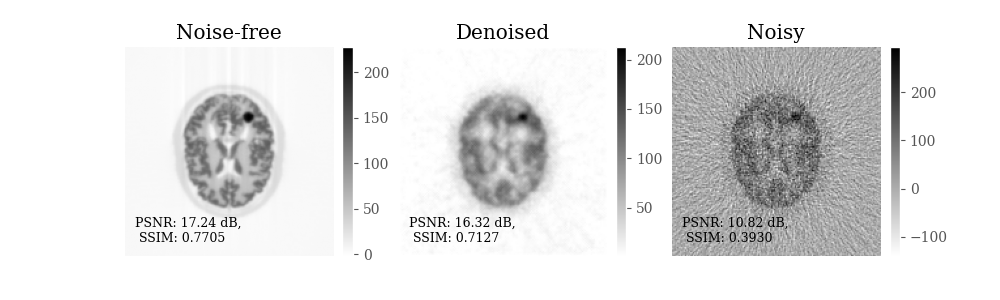
\includegraphics[scale=0.473]{image_to_image/results.png}
        \caption{Photon domain training results}
    \end{figure}
\end{frame}

\begin{frame}{Joint denoising and reconstruction}{Application to PET reconstruction}

    \centering
    \begin{tikzpicture}
        \tiny
        \node (full_sino) {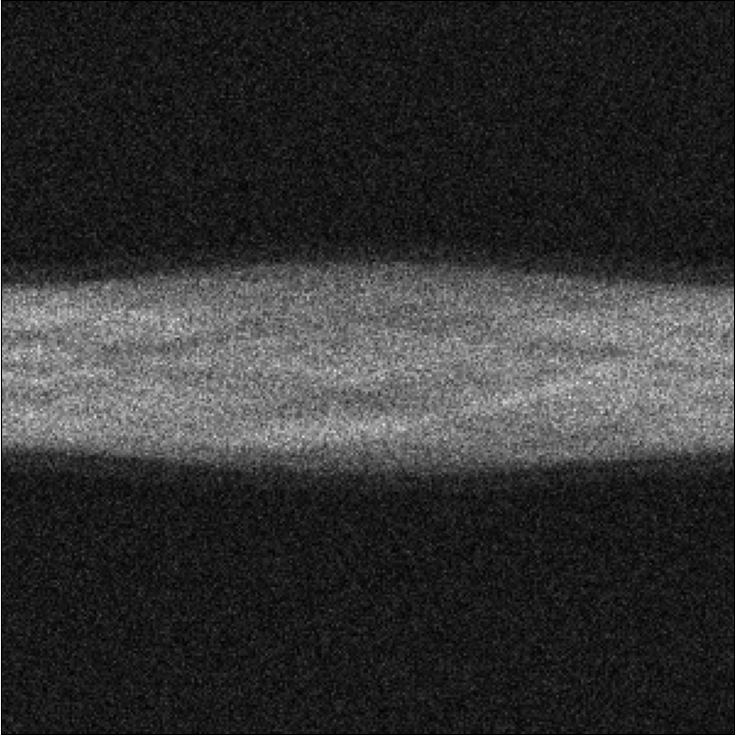
\includegraphics[scale=0.07]{photon_to_photon/sino_bin_0+1.png}};
        \node [right=0.1cm of full_sino] {Sampling};
        \node (bin0) [right=0.45cm of full_sino, yshift=-1.5cm] {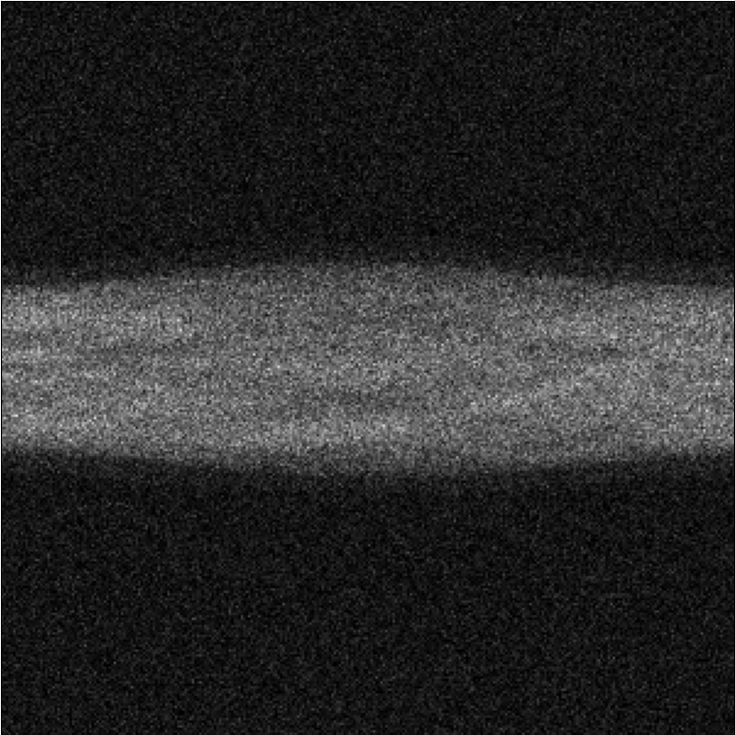
\includegraphics[scale=0.07]{photon_to_photon/sino_bin_0.png}};
        \node (bin1) [right=0.45cm of full_sino, yshift=1.5cm] {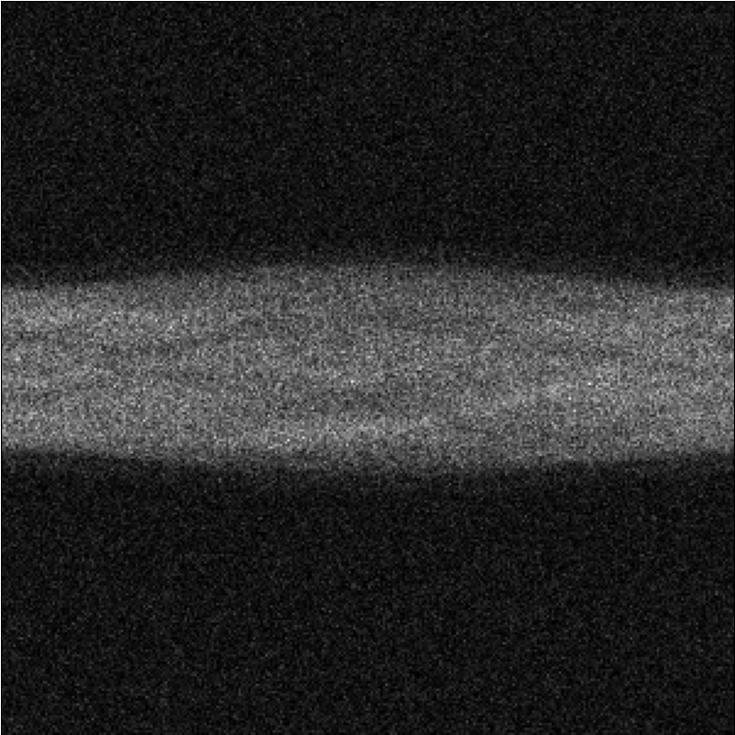
\includegraphics[scale=0.07]{photon_to_photon/sino_bin_1.png}};

        \node (recon_bin_0) [right=0.45cm of bin0] {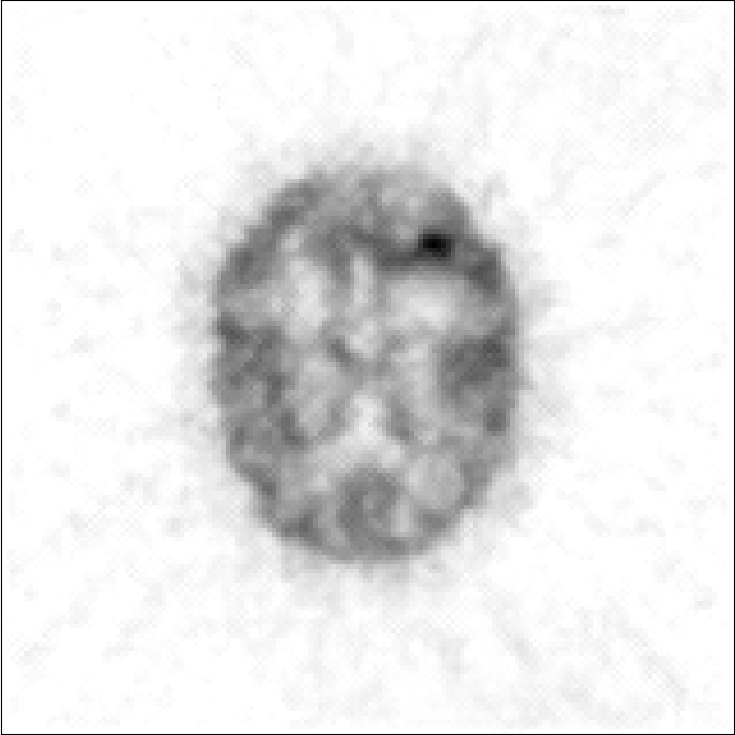
\includegraphics[scale=0.07]{image_to_image/brain_0_denoised.png}};
        \node (recon_bin_1) [right=0.45cm of bin1] {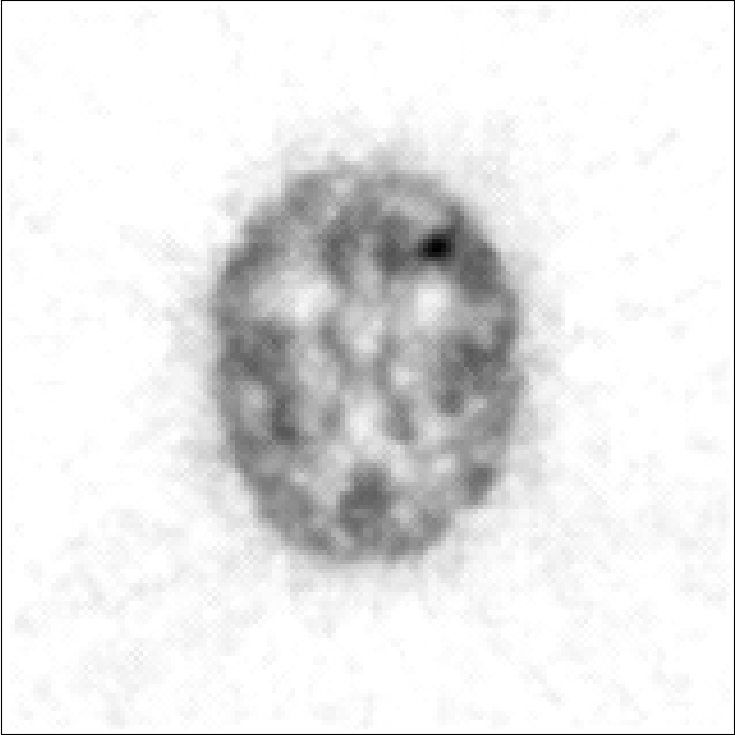
\includegraphics[scale=0.07]{image_to_image/brain_1_denoised.png}};

        \node (recon_full) [right=0.45cm of recon_bin_1, yshift=-1.5cm] {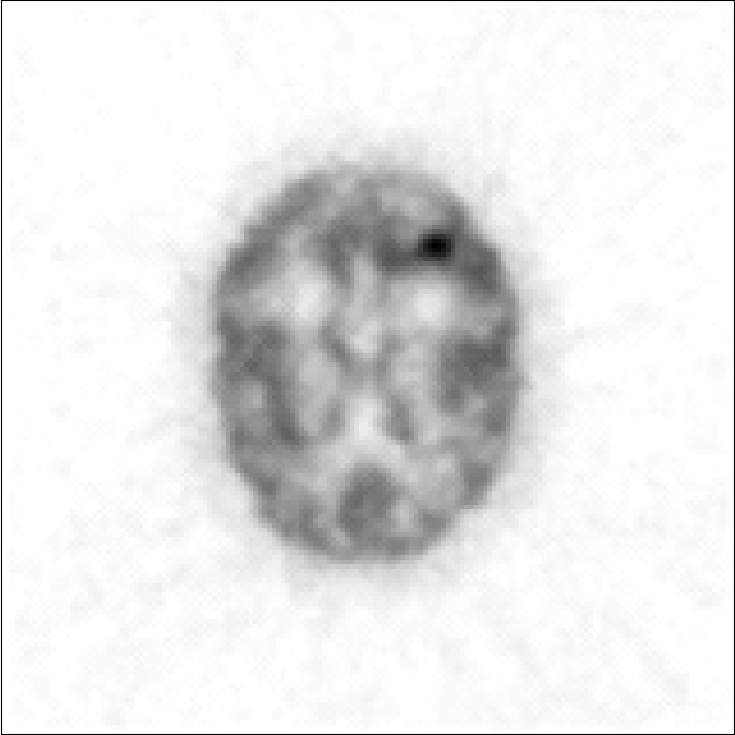
\includegraphics[scale=0.07]{image_to_image/brain_0+1_denoised.png}};

        \draw[->, thick] (full_sino) -- (bin0);
        \draw[->, thick] (full_sino) -- (bin1);
        \draw[->, thick] (bin0) -- (recon_bin_0) node[midway, below] {CNN};
        \draw[->, thick] (bin1) -- (recon_bin_1) node[midway, above] {CNN};
        \draw[->, thick] (recon_bin_0) -- (recon_full);
        \draw[->, thick] (recon_bin_1) -- (recon_full);

        \draw[<->, thick, orange] (recon_bin_0.north) -- (bin1.south) node[midway, above, fill=white, inner sep=1pt, yshift=0.15cm] {$\mathcal{L}_{\text{n2n}}$};
        \draw[<->, thick, orange] (recon_bin_1.south) -- (bin0.north);

    \end{tikzpicture}
    
\end{frame}

\begin{frame}{Joint denoising and reconstruction}
    Work in Progress.
\end{frame}


\begin{frame}{References}
    \tiny
    \printbibliography
\end{frame}

\end{document}